\chapter{数值模拟}
我们采用计算机来求解模型.为了简化编程,我们主要采用MATLAB矩阵实验室进行有限差分法的数值计算.\par
\section{扩散方程的模拟}
我们考虑这样简单的扩散方程,
\begin{equation}
\begin{cases}
\dfrac{\partial u}{\partial t}=\dfrac{\partial^2 u}{\partial x^2}+2 & 0<x<1,t>0, \\
u(0,t)=u(1,t)=0,& t>1, \\
u(x,0)=sin(\pi x)+x(1-x).
\end{cases}
\end{equation}
我们采用六点差分格式来解这个方程,下面为用MATLAB编写的计算程序.
 \begin{lstlisting}[caption=六点差分格式,language=Matlab]
function [e]=six(dx,dt,t)
    m=1/dx;
    n=t/dt;
    u1=zeros(1,m+1);
    x=[1:m-1]*dx;
    u1([2:m])= sin(pi*x)+x.*(1 - x);
    r=dt/dx/dx;r2=2+2*r;r3=2-2*r;
    for i=1:m-1
	a(i,i)=r2;if i>1
	a(i-1,i)=-r;
	a(i,i-1)=-r;
	end;
    end
    for i=1:m-1
	b(i,i)=r3;
	if i>1
	    b(i-1,i)=r;
	    b(i,i-1)=r;
	end
    end
    u=zeros(n+1,m+1);
    u(n+1,:)=u1;
    for k=1:n
	b=b*(u(n+2-k,2:m))'+0.04;
	u(n+1-k,2:m)=inv(a)*b;
    end
    ut=u(1,:);
    x1=[0,x,1];
    plot(x1,ut,'*')
\end{lstlisting}
\begin{figure}[h]
 \centering
 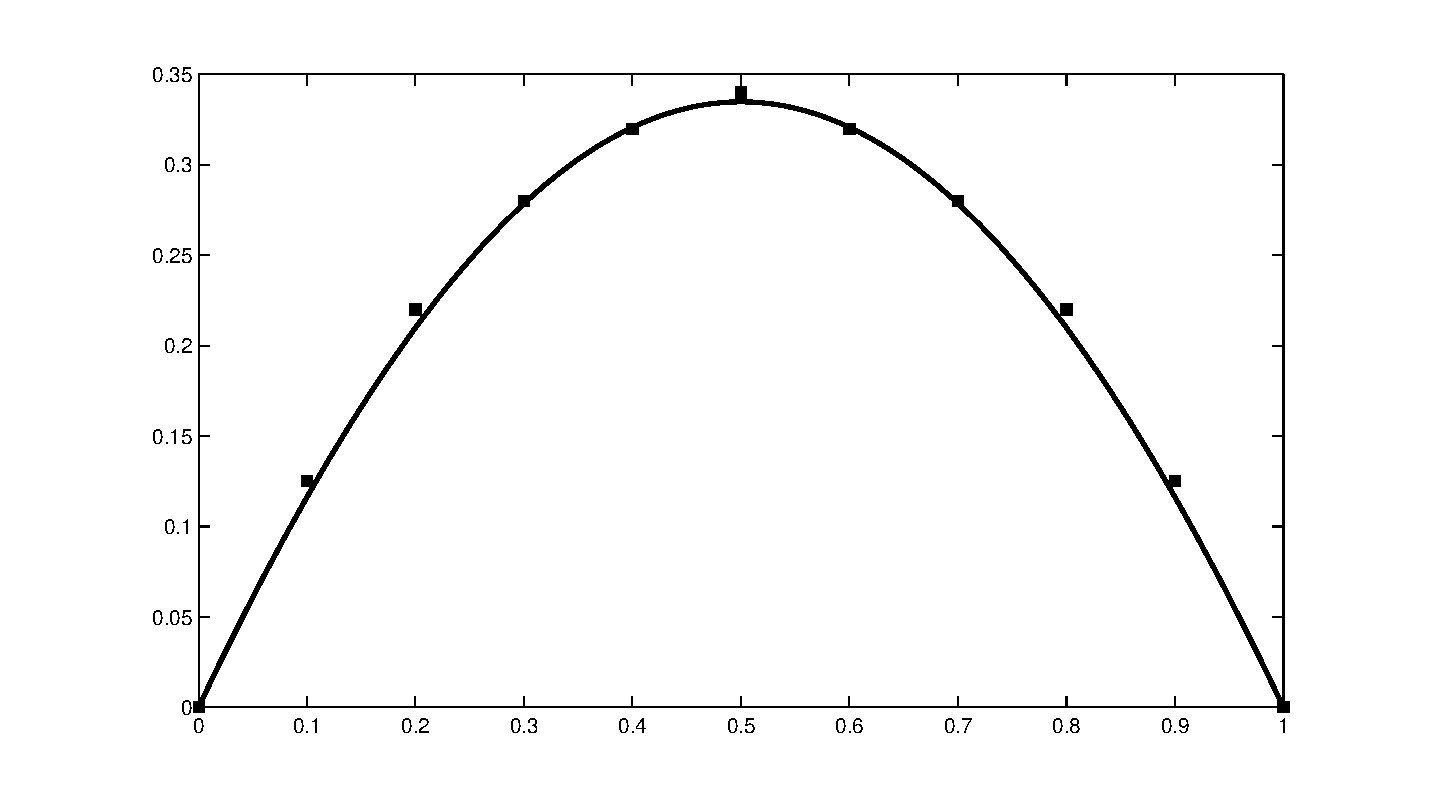
\includegraphics[scale=0.5]{./pic/6dcf.eps}
 \caption{扩散方程六点差分格式计算结果\label{fig:sm_ldcf}}
\end{figure}\par
仿真结果如图~\ref{fig:sm_ldcf}~所示,图中方块表示差分的数值结果,曲线表示解析结果.可以看到,虽然差分结果相对于解析解
是有误差的,但是误差不是很大.\newpage
\section{对流扩散方程的模拟}
考虑对流扩散方程
\begin{equation}\label{equ:cf_dkfangc}
	\dfrac{\partial u}{\partial t}+a\dfrac{\partial u}{\partial x}=\nu\dfrac{\partial^2 u}{\partial x^2}
\end{equation}
其中a、$\nu$ 为常数,$\nu>0$,给定初值
\begin{equation}
	u(x,0)=g(x)
\end{equation}
我们利用差分方法得到了一组差分方程,然后利用追赶法求解.
\begin{lstlisting}[caption=对流扩散方程差分求解,language=Matlab]
function C_k_1 = pencur3(Cin,u,A,B,D,E)
  M=2000;N=50;
  C_0=zeros(N+1,1);
  C_k_1=zeros(N+1,M);
  T=2500;L=40;
  t=T/M;
  h=L/N;
  a=B-2*A*u*h/D;
  AA=zeros(N+1);
  AA(1,1)=a;AA(1,2)=E+A;
  AA(N+1,N)=A+E;AA(N+1,N+1)=B;
  for i=2:N
      AA(i,i-1)=A;
      AA(i,i)=B;
      AA(i,i+1)=E;	
  end
  R=C_0;
  Rplus =-2*h*u*A/D*[1;zeros(N,1)];
  C_k_1(:,1)=C_0;
  for i=2:M
      R=C_k_1(:,i-1)+Rplus;
      C_k_1(:,i)=AA\R;
  end
  c=C_k_1;
  plot([1:M]',c(N+1,:));
  title('Curve');
  xlabel('t');
  ylabel('C/Cin');
end
\end{lstlisting}

\begin{figure}[h]
\centering
 \begin{floatrow}
 \ffigbox{\caption{对流扩散方程的差分计算结果1\label{fig:sm_dlfc1}}}{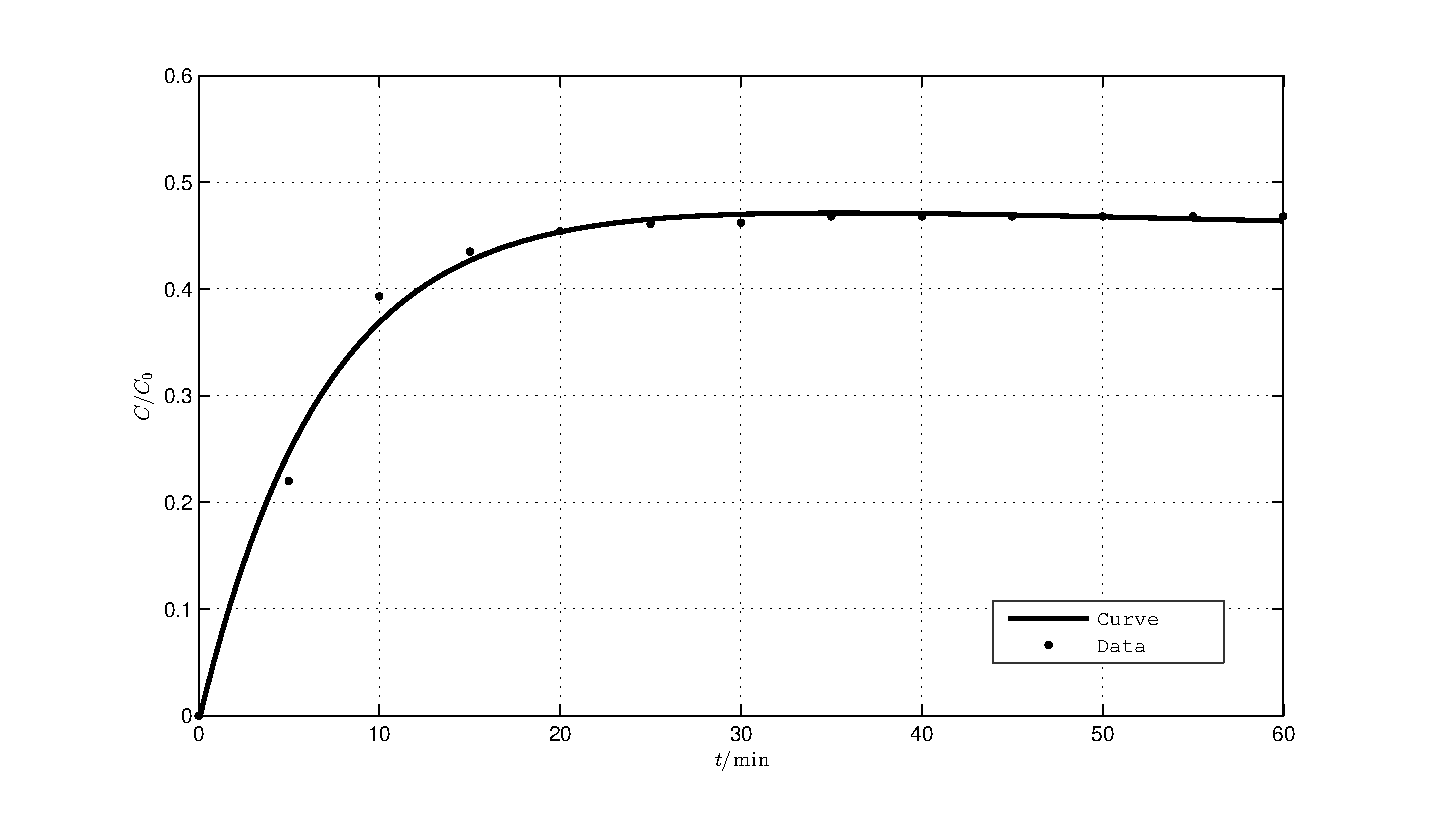
\includegraphics[scale=0.3]{./pic/dlfc.eps}}
 \ffigbox{\caption{对流扩散方程的差分计算结果2\label{fig:sm_dlfc2}}}{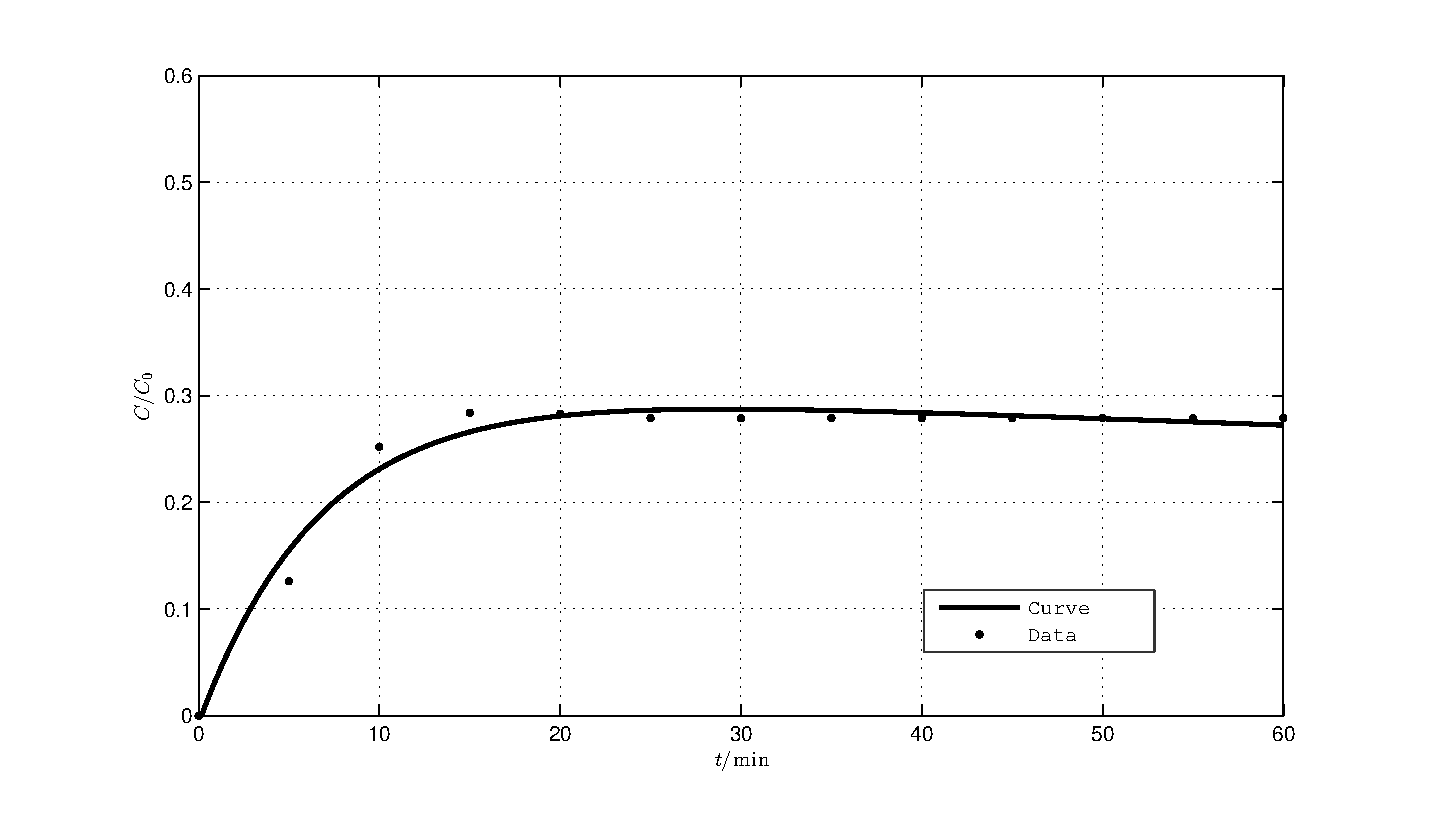
\includegraphics[scale=0.3]{./pic/dlfc2.eps}}
 \end{floatrow}
\end{figure}
% \begin{figure}[h]
%  \centering
%  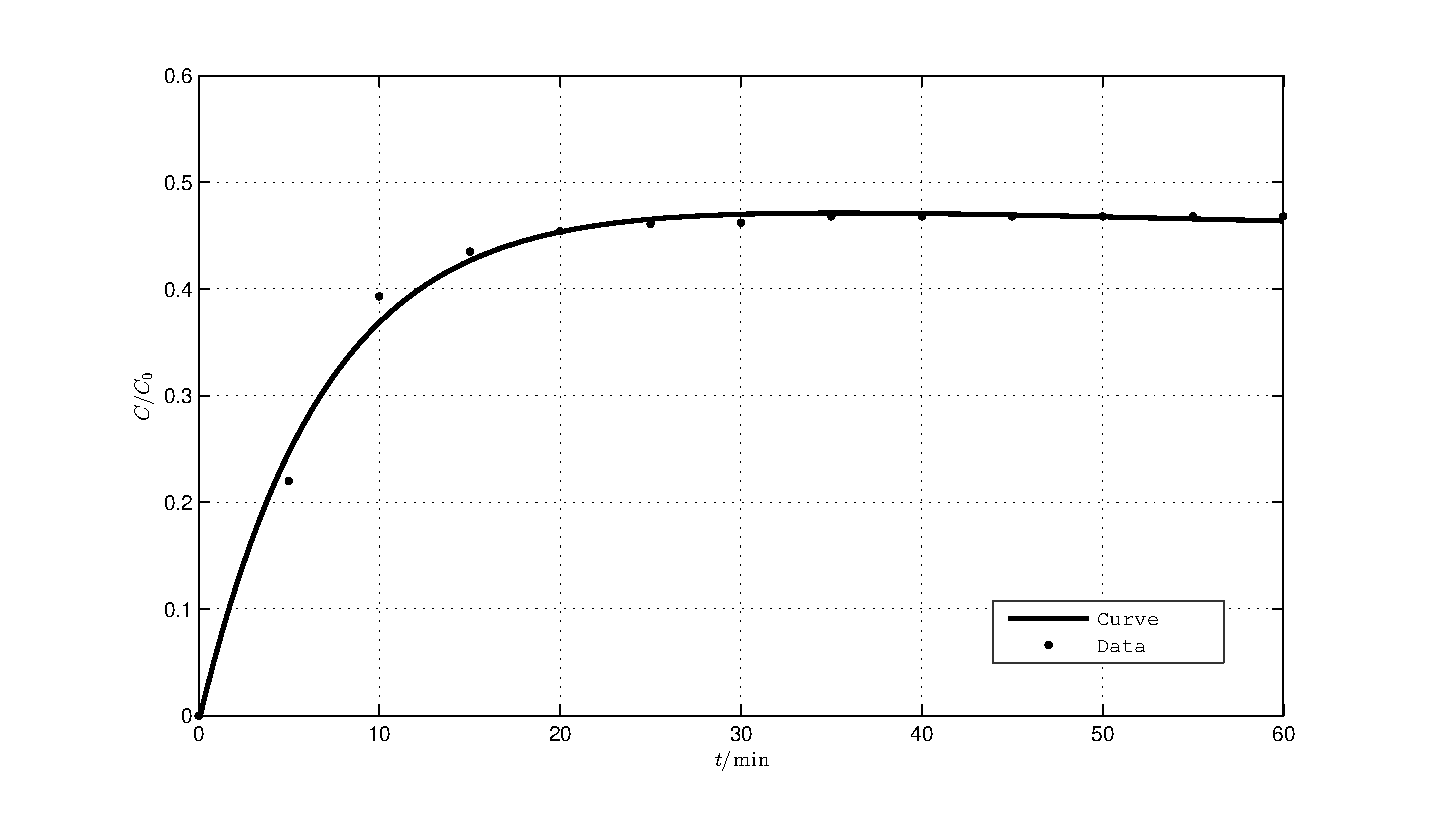
\includegraphics[scale=0.65]{./pic/dlfc.eps}
%  \caption{对流扩散方程(迎风格式)的差分计算结果1\label{fig:sm_dlfc}}
% \end{figure}\par
% \begin{figure}[h]
%  \centering
%  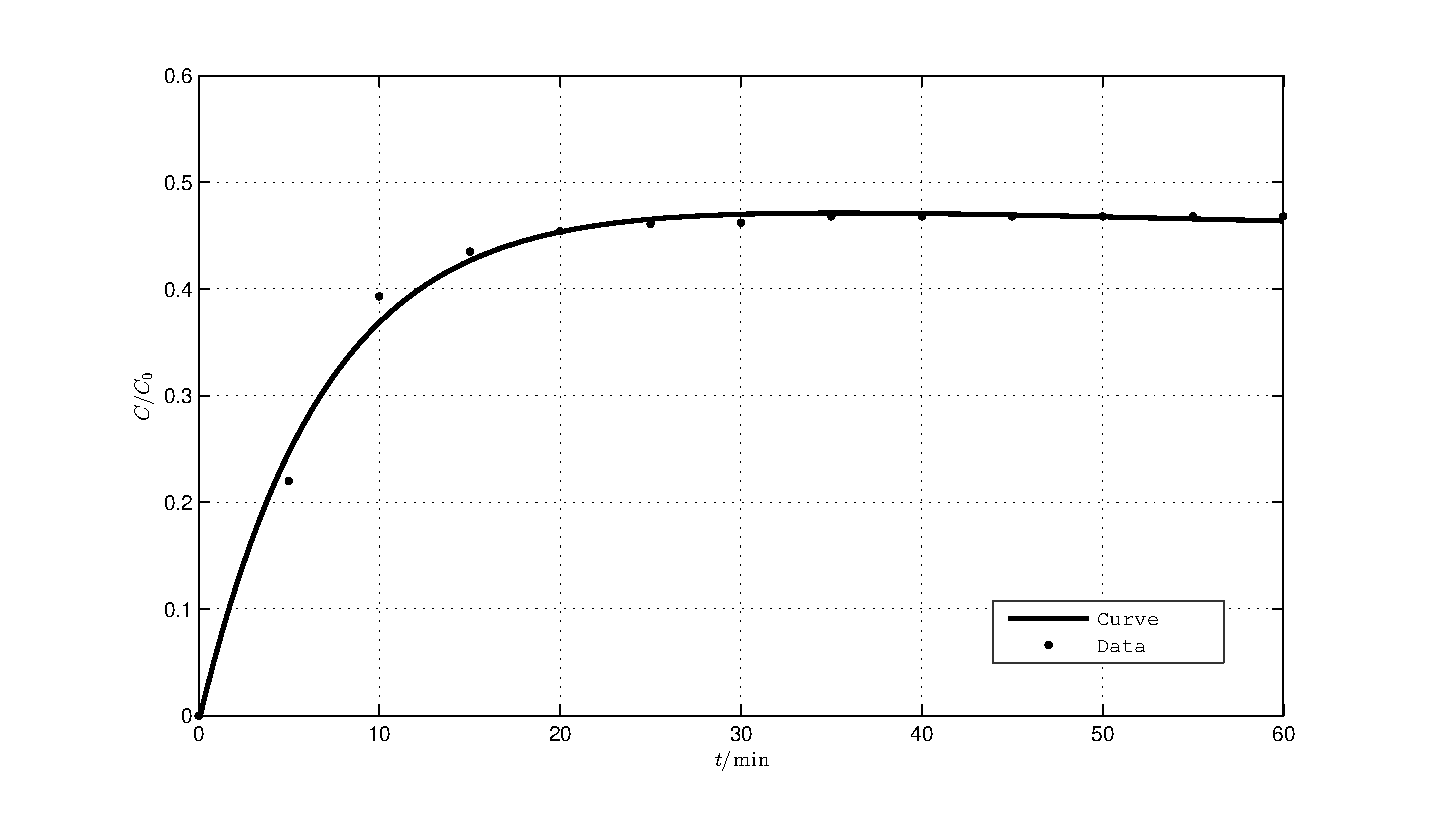
\includegraphics[scale=0.65]{./pic/dlfc.eps}
%  \caption{对流扩散方程(迎风格式)的差分计算结果2\label{fig:sm_dlfc2}}
% \end{figure}\par
图~\ref{fig:sm_dlfc1}~和图~\ref{fig:sm_dlfc2}~是对流扩散方程采用迎风格式的差分计算结果.其中,图线表示计算结果,方块是实验结果.我们看到,
模型在这个参数下可以较好地模拟实际的扩散情况.
\section{多维方程的模拟}
考虑这样的多维方程
\begin{equation}\label{eq:sm_dw}
R_d\dfrac{\partial C}{\partial t}+v_i\dfrac{\partial C}{\partial x_i}=\dfrac{\partial}{\partial x_i}(D_{ij}\dfrac{\partial C}
{\partial x_j})-\mu C+\lambda,\quad (i,j=1,2)
\end{equation}
我们采用有限元法来求解这个方程,不考虑对流项,利用MATLAB工具箱,程序如下
\begin{lstlisting}[caption=有限元法,language=Matlab]
function pdemodel
[pde_fig,ax]=pdeinit;
pdetool('appl_cb',1);
set(ax,'DataAspectRatio',[1 0.0060000000000000001 1]);
set(ax,'PlotBoxAspectRatio',[250 166.66666666666666 50]);
set(ax,'XLim',[0 10]);
set(ax,'YLim',[-0.02 0.02]);
set(ax,'XTickMode','auto');
set(ax,'YTickMode','auto');

pderect([0 10 0.0050000000000000001 -0.0050000000000000001],'R1');
set(findobj(get(pde_fig,'Children'),'Tag','PDEEval'),'String','R1')

pdetool('changemode',0)
pdesetbd(4,...
'dir',...
1,...
'1',...
'6e8')
pdesetbd(3,...
'neu',...
1,...
'0',...
'0')
pdesetbd(2,...
'neu',...
1,...
'0',...
'0')
pdesetbd(1,...
'neu',...
1,...
'0',...
'0')

setappdata(pde_fig,'Hgrad',1.3);
setappdata(pde_fig,'refinemethod','regular');
setappdata(pde_fig,'jiggle',char('on','mean',''));
pdetool('initmesh')
pdetool('refine')
pdetool('refine')

pdeseteq(2,...
'3.66e-6',...
'1.035e-3',...
'7.819e5',...
'1.0',...
'0:10',...
'0.0',...
'0.0',...
'[0 100]')
setappdata(pde_fig,'currparam',...
['3.66e-6 ';...
'1.035e-3';...
'7.819e5 ';...
'1.0     '])

setappdata(pde_fig,'solveparam',...
str2mat('0','2016','10','pdeadworst',...
'0.5','longest','0','1E-4','','fixed','Inf'))

setappdata(pde_fig,'plotflags',[1 1 1 1 1 1 1 1 0 0 0 11 1 0 0 0 0 1]);
setappdata(pde_fig,'colstring','');
setappdata(pde_fig,'arrowstring','');
setappdata(pde_fig,'deformstring','');
setappdata(pde_fig,'heightstring','');
pdetool('solve')
\end{lstlisting}\par
模拟的结果如彩图~\ref{pic:simu_1}~、~\ref{pic:simu_2}、~\ref{pic:simu_3}~、~\ref{pic:simu_4}~、~\ref{pic:simu_5}~、
~\ref{pic:simu_6}~所示.可以看到,微生物在随着时间的推进而向着深度增加而向内部扩散.这与实际的情况是相符的.
% \newpag
\section{本章小节}
本章利用计算机对数值算法进行了模拟和仿真.利用了第二章中检索得到的数学模型对数值算法进行了计算和验证.仿真结果证明,
我们所采用的数值计算方法是简单而有效的,运算速度快,效率高.